%!TEX root = ../User Guide.tex
\chapter{Introduction and overview}
CACTUS (\textbf{C}ode for \textbf{A}xial and \textbf{C}rossflow \textbf{TU}rbine \textbf{S}imulation) is a turbine performance simulation code using a blade element discretization and a free vortex line description of the turbine wake. The code was originally based on \path{VDART3}, a free vortex wake simulation of the Darrieus wind turbine, developed by Strickland \cite{Strickland1979}. The codebase has been largely upgraded to the Fortran 9x standard, and a number of modifications have been made to the original \path{VDART3} methods including updates to the blade loads models, and new models to handle generic device geometry and marine turbine specific physics.

This document serves as a user's manual for CACTUS. A brief overview of the code is provided below, however, more detailed information on the methods used can be found in \cite{Murray2011}. 

\section{Blade loads and wake models}
CACTUS simulates a turbine device consisting of an arbitrary configuration of blade element sections. Each section can be assigned arbitrary load coefficient vs. angle of attack characteristics, which typically correspond to two-dimensional lift and drag coefficient data for a particular foil section. Since data from two-dimensional wind tunnel tests or foil performance calculations are used to represent element loads, it is generally assumed that these elements are in locally two-dimensional flow. 

A rotor blade consisting of an arbitrary planform shape and foil sections can be modeled by the synthesis of a number of blade elements. The blade loads and wake of the turbine rotor are evolved in time over a certain number of rotor revolutions, until the revolution-averaged rotor power is converged.  The code output includes the blade aerodynamic forces, wake vortex trajectories, and performance metrics such as torque and power.  

CACTUS uses a potential flow model comprised of free vortex line elements to represent the turbine wake flow field. The vortex line structure attached to a single blade element is shown in \Cref{fig:vortex_lattice}. At each point in time, the bound vorticity ($\Gamma_B$) on each blade element is related to the element lift coefficient through the Kutta-Joukowski theorem, and the spanwise ($\Gamma_S$) and trailing vorticity ($\Gamma_T$) are recovered through the application of the Helmholz theorem of conservation of circulation along a vortex line \cite{katz2001low}.

\begin{figure}
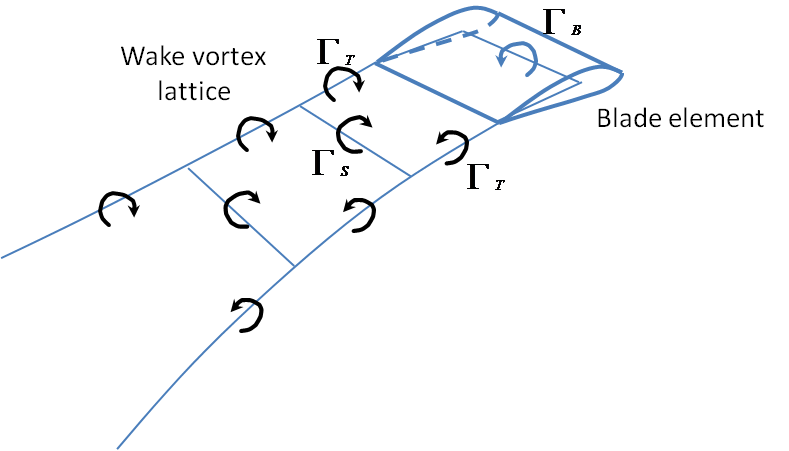
\includegraphics{figures/vortex_lattice.png}
\label{fig:vortex_lattice}
\caption{Blade element with associated vortex lattice system.}
\end{figure}

\subsection{Dynamic blade loads}
The operational cycle of some turbines, most notably cross-flow turbines or axial flow turbines in yawed flow conditions, cause the turbine blades to operate in dynamically variable flow conditions. The effects of blade rotation with respect to the surrounding fluid and the effects of dynamically variable flow angle of attack are captured with additional models.

The effects of blade section pitch rate (rotation around an axis normal to the section plane) are captured by analogy to an analytical solution for a pitching flat plate. Improvements have been made to the original methodology used in \path{VDART3}, and modifications have been made to handle non-zero section pitching moment due to cambered foil sections.

Under certain operational conditions, the turbine blades may operate at angles of attack beyond their steady-state stall limits for significant lengths of time. The transient behavior of the blade section loads during this ``dynamic stalling'' process must be modeled as it is not captured by the steady load coefficient data input for each foil section. The primary effect of dynamic stalling is a delay in the appearance of stalled flow effects on blade loads to higher angles of attack than would be expected in steady flow.

Two models for dynamic stall effects on blade section loads are included in CACTUS. The modified Boeing-Vertol method of Gormont is the default. This algebraic method approximates dynamic stall effects with a ``lagged'' angle of attack, where the magnitude of the lag is empirically correlated to the angle of attack rate. The Leishman-Beddoes model incorporates more physical models and attempts to model the temporal evolution of dynamic stall flow phenomena and associated effects on blade loads. This model may provide more accurate results than the algebraic Boeing-Vertol method, but requires many more simulation time steps to be taken per turbine revolution to achieve converged results.

\section{Solid and free-surface boundaries}
CACTUS can simulate the effects of proximity to a ground plane or free (water) surface on turbine performance. The boundary conditions, either zero normal flow for a ground plane or constant surface pressure for a free surface, are applied using rectangular source panel elements. The free surface boundary condition is currently implemented as a quasi-static boundary, allowing it to respond only to the average flow created by the turbine and wake over a full revolution. 

The user is allowed to specify the time step interval between updates to the wall panel system. For the free surface model, the wall update interval specifies the number of time steps between updates to the revolution averaged quantities. It is often not necessary to update these quantities on every time step. If it's possible to reduce the frequency of wall panel system updates and still obtain convergence of the simulation output of interest, this can reduce simulation run time considerably.

A recent addition to CACTUS is the ability to model \emph{general} solid boundaries, or walls, using generalized quadrilateral source panels. A 3-D mesh file describing the wall geometry must be generated externally and passed as an input to CACTUS.